% BibTeX entries live here; this block writes them to build/references.bib at compile time.
\begin{filecontents*}[overwrite]{references.bib}
@inproceedings{cammerer2023,
  title={A Neural Receiver for {5G NR} Multi-user {MIMO}},
  author={Cammerer, Sebastian and A{\"i}t Aoudia, Fay{\c{c}}al and Hoydis, Jakob and Oeldemann, Andreas and Roessler, Andreas and Mayer, Timo and Keller, Alexander},
  booktitle={Proc. IEEE Globecom Workshops},
  pages={329--334},
  year={2023}
}
@article{wiesmayr2024,
  title={Design of a Standard-Compliant Real-Time Neural Receiver for {5G NR}},
  author={Wiesmayr, Reinhard and Cammerer, Sebastian and A{\"i}t Aoudia, Fay{\c{c}}al and Hoydis, Jakob and Zakrzewski, Jakub and Keller, Alexander},
  journal={arXiv preprint arXiv:2409.02912},
  year={2024}
}
@article{hoydis2022,
  title={Sionna: An Open-Source Library for Next-Generation Physical Layer Research},
  author={Hoydis, Jakob and Cammerer, Sebastian and A{\"i}t Aoudia, Fay{\c{c}}al and Vem, Avinash and Binder, Nikolaus and Marcus, Guillermo and Keller, Alexander},
  journal={arXiv preprint arXiv:2203.11854},
  year={2022}
}
@techreport{tr38901,
  title={Study on Channel Model for Frequencies from 0.5 to 100 {GHz}},
  author={{ETSI}},
  number={3GPP TR 38.901, Release 16.1},
  institution={ETSI},
  year={2020}
}
@inproceedings{hoydis2023,
  title={Sionna {RT}: Differentiable Ray Tracing for Radio Propagation Modeling},
  author={Hoydis, Jakob and A{\"i}t Aoudia, Fay{\c{c}}al and Cammerer, Sebastian and Nimier-David, Merlin and Binder, Nikolaus and Marcus, Guillermo and Keller, Alexander},
  booktitle={Proc. IEEE Globecom Workshops},
  pages={317--321},
  year={2023}
}
@book{dahlman2020,
  title={{5G NR}: The Next Generation Wireless Access Technology},
  author={Dahlman, Erik and Parkvall, Stefan and Sk{\"o}ld, Johan},
  publisher={Academic Press},
  year={2020}
}
@techreport{ts38214,
  title={Physical Layer Procedures for Data},
  author={{ETSI}},
  type={Technical Specification},
  number={ETSI TS 138 214 V16.2.0},
  institution={ETSI},
  year={2020}
}
@article{hochwald2003,
  title={Achieving Near-Capacity on a Multiple-Antenna Channel},
  author={Hochwald, Bertrand M. and ten Brink, Stephan},
  journal={IEEE Transactions on Communications},
  volume={51},
  number={3},
  pages={389--399},
  year={2003}
}
@article{richardson2018,
  title={Design of Low-Density Parity Check Codes for {5G} New Radio},
  author={Richardson, Tom and Kudekar, Shrinivas},
  journal={IEEE Communications Magazine},
  volume={56},
  number={3},
  pages={28--34},
  year={2018}
}
@article{guo2006,
  title={Algorithm and Implementation of the {K}-Best Sphere Decoding for {MIMO} Detection},
  author={Guo, Zhan and Nilsson, Peter},
  journal={IEEE Journal on Selected Areas in Communications},
  volume={24},
  number={3},
  pages={491--503},
  year={2006}
}
@inproceedings{kingma2015,
  title={Adam: A Method for Stochastic Optimization},
  author={Kingma, Diederik P. and Ba, Jimmy},
  booktitle={Proc. International Conference on Learning Representations (ICLR)},
  year={2015}
}
\end{filecontents*}
\documentclass[letterpaper]{article} % DO NOT CHANGE THIS
\usepackage[submission]{aaai2027}  % DO NOT CHANGE THIS
% The serif, sans-serif, and monospaced fonts are loaded automatically by
% aaai2027.sty (newtxtext, helvet, courier). DO NOT add \usepackage{times},
% \usepackage{helvet}, \usepackage{courier}, or any other font package.
\usepackage[hyphens]{url}  % DO NOT CHANGE THIS
\usepackage{graphicx} % DO NOT CHANGE THIS
\urlstyle{rm} % DO NOT CHANGE THIS
\def\UrlFont{\rm}  % DO NOT CHANGE THIS
\usepackage{natbib}  % DO NOT CHANGE THIS AND DO NOT ADD ANY OPTIONS TO IT
\usepackage{caption} % DO NOT CHANGE THIS AND DO NOT ADD ANY OPTIONS TO IT
\frenchspacing  % DO NOT CHANGE THIS
%
% These are recommended to typeset algorithms but not required. See the subsubsection on algorithms. Remove them if you don't have algorithms in your paper.
\usepackage{algorithm}
\usepackage{algorithmic}

%
% These are recommended to typeset listings but not required. See the subsubsection on listing. Remove this block if you don't have listings in your paper.
\usepackage{newfloat}
\usepackage{listings}
\DeclareCaptionStyle{ruled}{labelfont=normalfont,labelsep=colon,strut=off} % DO NOT CHANGE THIS
\lstset{%
	basicstyle={\footnotesize\ttfamily},% footnotesize acceptable for monospace
	numbers=left,numberstyle=\footnotesize,xleftmargin=2em,% show line numbers, remove this entire line if you don't want the numbers.
	aboveskip=0pt,belowskip=0pt,%
	showstringspaces=false,tabsize=2,breaklines=true}
\floatstyle{ruled}
\newfloat{listing}{tb}{lst}{}
\floatname{listing}{Listing}

%
% Recommended for better-looking tables
\usepackage{booktabs}
\usepackage{amsmath}
\usepackage{amssymb}

%
% Keep the \pdfinfo as shown here. There's no need
% for you to add the /Title and /Author tags.
\pdfinfo{
/TemplateVersion (2027.1)
}

% DISALLOWED PACKAGES
% \usepackage{authblk} -- This package is specifically forbidden
% \usepackage{balance} -- This package is specifically forbidden
% \usepackage{CJK} -- This package is specifically forbidden
% \usepackage{float} -- This package is specifically forbidden
% \usepackage{flushend} -- This package is specifically forbidden
% \usepackage{fullpage} -- This package is specifically forbidden
% \usepackage{geometry} -- This package is specifically forbidden
% \usepackage{hyperref} -- This package is specifically forbidden
% \usepackage{navigator} -- This package is specifically forbidden
% (or any other package that embeds links such as navigator or hyperref)
% \usepackage{indentfirst} -- This package is specifically forbidden
% \usepackage{layout} -- This package is specifically forbidden
% \usepackage{multicol} -- This package is specifically forbidden
% \usepackage{nameref} -- This package is specifically forbidden
% \usepackage{savetrees} -- This package is specifically forbidden
% \usepackage{setspace} -- This package is specifically forbidden
% \usepackage{stfloats} -- This package is specifically forbidden
% \usepackage{tabu} -- This package is specifically forbidden
% \usepackage{titlesec} -- This package is specifically forbidden
% \usepackage{tocbibind} -- This package is specifically forbidden
% \usepackage{ulem} -- This package is specifically forbidden
% \usepackage{wrapfig} -- This package is specifically forbidden
% DISALLOWED COMMANDS
% \nocopyright -- Your paper will not be published if you use this command
% \addtolength -- This command may not be used
% \balance -- This command may not be used
% \baselinestretch -- Your paper will not be published if you use this command
% \clearpage -- No page breaks of any kind may be used for the final version of your paper
% \columnsep -- This command may not be used
% \newpage -- No page breaks of any kind may be used for the final version of your paper
% \pagebreak -- No page breaks of any kind may be used for the final version of your paper
% \pagestyle -- This command may not be used
% \tiny -- This is not an acceptable font size.
% \vspace{- -- No negative value may be used in proximity of a caption, figure, table, section, subsection, subsubsection, or reference
% \vskip{- -- No negative value may be used to alter spacing above or below a caption, figure, table, section, subsection, subsubsection, or reference

\setcounter{secnumdepth}{0} %May be changed to 1 or 2 if section numbers are desired.

% The file aaai2027.sty is the style file for AAAI Press
% proceedings, working notes, and technical reports.
%

% Title

% Your title must be in mixed case, not sentence case.
% That means all verbs (including short verbs like be, is, using,and go),
% nouns, adverbs, adjectives should be capitalized, including both words in hyphenated terms, while
% articles, conjunctions, and prepositions are lower case unless they
% directly follow a colon or long dash
\title{A Neural Receiver with Per-UE Pilot Memory for 5G NR Multi-user MIMO}
\author{
    Anonymous Authors
}
\affiliations{
    Anonymous Affiliation
}

\begin{document}

\maketitle

\begin{abstract}
% TODO: abstract, once the paper's direction is decided.
Abstract to be written.
\end{abstract}

\section{Introduction}
% TODO: introduction, once the paper's direction is decided.

\section{Receiver Design}

\subsection{System Model}
We consider multi-user multiple-input multiple-output (MU-MIMO) uplink transmission from $U$ user equipments (UEs) to a base station (BS) with $B$ antennas over the 5G NR physical uplink shared channel (PUSCH)~\cite{dahlman2020}. Each slot carries one transport block (TB) per scheduled UE on an orthogonal frequency division multiplexing (OFDM) resource grid with $S$ subcarriers and $T=14$ OFDM symbols. The received signal on subcarrier $s$ and OFDM symbol $t$ is
\begin{equation}
\mathbf{y}_{s,t}=\sum_{u=1}^{U}\mathbf{h}_{s,t,u}\,x_{s,t,u}+\mathbf{n}_{s,t},
\end{equation}
where $\mathbf{h}_{s,t,u}\in\mathbb{C}^{B}$ is the effective channel of UE $u$ after beamforming, $x_{s,t,u}$ is its modulated symbol or pilot, and $\mathbf{n}_{s,t}\sim\mathcal{CN}(\mathbf{0},N_0\mathbf{I})$ is complex Gaussian noise with power spectral density $N_0$. Demodulation reference signal (DMRS) positions are fixed, but the DMRS sequence depends on the slot number. The receiver computes log-likelihood ratio (LLR) estimates for each coded bit $b$ of each UE. We define the LLRs as logits, i.e.,
\begin{equation}
\ell=\ln\frac{\Pr(b=1\,|\,\mathbf{Y})}{\Pr(b=0\,|\,\mathbf{Y})},
\end{equation}
where $\mathbf{Y}$ collects all $\mathbf{y}_{s,t}$ of the slot. The LLR estimates are fed to the channel decoder.

\subsection{Neural Receiver}
We build on the neural receiver (NRX) of \citet{cammerer2023} and \citet{wiesmayr2024}, which combines convolutional and graph neural network (CGNN) layers. A least squares (LS) channel estimate initializes the \texttt{StateInit} layer, $N_{\mathrm{it}}$ \texttt{CGNNIt} blocks update the state of each UE, and \texttt{ReadoutLLRs} outputs the LLRs. This NRX processes each slot independently. We call the version with $N_{\mathrm{it}}=8$ the \emph{Large NRX}.

Each CGNN iteration adds latency~\cite{wiesmayr2024}. The proposed NRX, shown in Fig.~\ref{fig:architecture}, therefore uses $N_{\mathrm{it}}=2$ and compensates for the fewer iterations with a pilot memory, a channel filter, and iterative detection and decoding (IDD). It has $1.4\cdot 10^{5}$ weights, of which only 643 are new, compared with $4.4\cdot 10^{5}$ for the Large NRX.

\begin{figure*}[t]
\centering
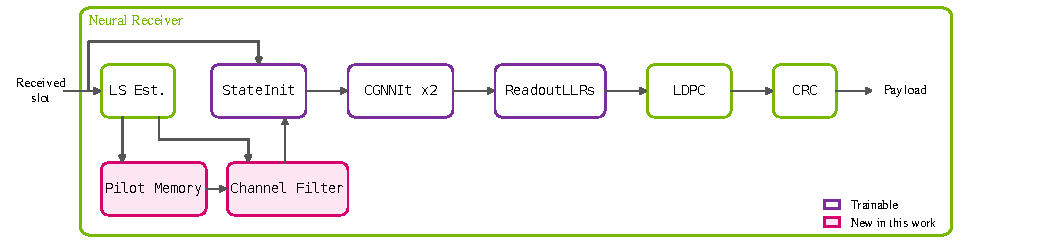
\includegraphics[width=\textwidth]{figures/receiver_architecture.pdf}
\caption{Proposed NRX for 5G NR PUSCH.}
\label{fig:architecture}
\end{figure*}

\subsection{Pilot Memory}
The channel of a UE evolves over consecutive slots, but an NRX that processes each slot independently discards all earlier pilots. Earlier pilots carry information on how the channel changes over time, which the few DMRS symbols of a single slot capture only partially on fast-varying channels. We therefore store the LS channel estimates at each UE's DMRS positions, together with $N_0$, for up to seven previous TBs. Entries older than eight slots (4\,ms at 30\,kHz subcarrier spacing) are ignored, as they are likely outdated. A UE returning after a scheduling gap thus resumes from its recent entries, if any.

The memory is written from pilots only. Decoded bits and cyclic redundancy check (CRC) outcomes never enter it, so a decoding failure cannot corrupt later slots. It is also the only state kept across slots, and all weights stay frozen during operation. As in \citet{wiesmayr2024}, we do not assume training on-the-fly.

\subsection{Channel Filter}
A small learned filter refines the current LS estimate $\mathbf{h}_0\in\mathbb{C}^{B}$ of a DMRS position using nearby estimates $\mathbf{h}_j$, $j\in\mathcal{N}$, from the current TB and the memory. It fits a local first-order channel model,
\begin{equation}
\begin{aligned}
\hat{\mathbf{h}}_{s,t,u}&=\sum_{r=0}^{2}\phi_r(s,t)\,\boldsymbol{\theta}_r,\\
\boldsymbol{\theta}_r&=\delta_{r,0}\mathbf{h}_0+\sum_{j\in\mathcal{N}}\beta_{j,r}\left(\mathbf{h}_j-\mathbf{h}_0\right),
\end{aligned}
\end{equation}
where $\phi_0=1$, $\phi_1$ and $\phi_2$ are normalized offsets in time and frequency relative to the DMRS position of $\mathbf{h}_0$, and $\delta_{r,0}$ is the Kronecker delta. The first-order terms capture how the channel varies around each DMRS position. The best weighting depends on the noise level, the Doppler shift, and the age of each entry; a learned weighting adapts to these factors without requiring channel statistics. A multilayer perceptron (MLP) with one hidden layer of 16 units computes the coefficients $\beta_{j,r}$ from the correlation of each $\mathbf{h}_j$ with $\mathbf{h}_0$ and from its power, noise level, age, and position. The filter can fall back to the current estimate when the memory does not help. The refined estimate $\hat{\mathbf{h}}_{s,t,u}$ replaces the LS estimate at the input of \texttt{StateInit}. A second MLP with one hidden layer of 16 units estimates its error covariance $\boldsymbol{\Sigma}_{s,t,u}$, which quantifies the reliability of the estimate for the subsequent processing.

\subsection{Iterative Detection and Decoding}
With only two CGNN iterations, the NRX LLRs are less reliable, whereas the decoder has information about the code that the NRX does not use. IDD~\cite{hochwald2003} feeds this information back to detection. We perform one IDD iteration by splitting low-density parity-check (LDPC) belief propagation (BP) decoding~\cite{richardson2018} into two stages. Let $L$ denote the NRX LLR of a coded bit. After eight BP iterations, we evaluate, for $U=2$ UEs, all 256 pairs $\mathbf{x}=[x_1,x_2]^{\mathsf{T}}$ of 16-QAM symbols on each data resource element, which is feasible for this small number of UEs, with the Gaussian log-likelihood, up to a constant,
\begin{equation}
\ln\Lambda(\mathbf{x})=-\ln\det\mathbf{C}(\mathbf{x})-\mathbf{e}(\mathbf{x})^{\mathsf{H}}\mathbf{C}(\mathbf{x})^{-1}\mathbf{e}(\mathbf{x}),
\end{equation}
where $\mathbf{e}(\mathbf{x})=\mathbf{y}_{s,t}-\sum_u\hat{\mathbf{h}}_{s,t,u}x_u$ and $\mathbf{C}(\mathbf{x})=N_0\mathbf{I}+\sum_u|x_u|^2\boldsymbol{\Sigma}_{s,t,u}$. Here, $\mathbf{C}(\mathbf{x})$ accounts for channel estimation errors, whose effect grows with the symbol energy. Marginalizing these likelihoods gives an a posteriori probability (APP) LLR $P$. Repeating this with the extrinsic LLRs of the first BP stage as symbol priors gives a second APP LLR $Q$. With a learned scaling factor $\sigma\in(0,1)$ and the correction $\Delta=\sigma(Q-P)$, the input to the remaining BP iterations is
\begin{equation}
J=(1-a)(L+\Delta)+a(P+\Delta),
\end{equation}
where the per-bit LLR combining weight $a\in[0,1]$ comes from an MLP with one hidden layer of eight units. As $L$ and $P$ rely on different models, neither can be expected to be the better choice for every bit. BP then continues for ten iterations from $J$ and the retained BP messages, which avoids repeating the first eight iterations, for a total of 18 iterations. None of the IDD outputs enter the memory.

\subsection{Training}
We train all weights end-to-end, starting from the pre-trained Large NRX. Training uses simulated TB sequences rather than independent slots, which allows the filter to learn how the channel evolves. We perform $5\cdot 10^{3}$ training steps with the ADAM optimizer~\cite{kingma2015} and a learning rate of $10^{-4}$. Sequences of 8 to 64 slots use 3GPP tapped delay line (TDL), urban microcell (UMi), and urban macrocell (UMa) channels~\cite{tr38901} with Doppler shifts up to 400\,Hz. They include near-far UEs, as well as scheduling gaps and channel changes, which expose the receiver to missing and outdated memory entries. The loss has three terms. The first is the binary cross-entropy on $L$, on the posterior LLRs after the first BP stage, and on $J$, to obtain reliable LLRs at every stage. The second acts on the decoded payload LLRs. Since a TB fails if any of its bits is wrong, it averages their binary cross-entropy and a normalized log-sum-exp of $-(2b-1)\ell$ over the payload bits $b$ and their LLRs $\ell$, a smooth maximum that approximates a TB error. The third, weighted by 0.1, is the Gaussian negative log-likelihood of the true channel given $\hat{\mathbf{h}}_{s,t,u}$ and $\boldsymbol{\Sigma}_{s,t,u}$, and trains both the estimate and its covariance. To keep the receiver functional with no memory, each TB is decoded both with memory and with no memory, and the two losses are weighted $1:0.5$. We select the checkpoint on a separate validation dataset.

\section{Evaluation}

\subsection{Simulation Setup}
We evaluate all receivers with Sionna~\cite{hoydis2022} for $U=2$ UEs and $B=4$ BS antennas, denoted $U\times B\equiv 2\times 4$, in the configuration of \citet{wiesmayr2024}: dual-polarized BS antennas with 3GPP TR 38.901 patterns~\cite{tr38901}, two single-polarized omnidirectional antennas per UE with beamforming $\mathbf{v}=[1,1]^{\mathsf{T}}/\sqrt{2}$, 132 physical resource blocks with 30\,kHz subcarrier spacing at a carrier frequency of 2.14\,GHz, modulation and coding scheme (MCS) index $i=14$ (16-QAM)~\cite[Table~5.1.3.1-1]{ts38214}, and DMRS type A with one additional position.

\begin{figure*}[t]
\centering
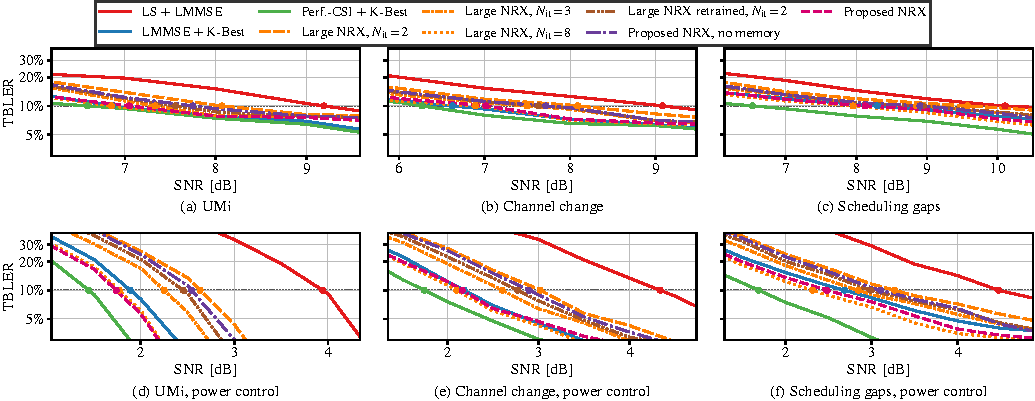
\includegraphics[width=\textwidth]{figures/tbler_vs_snr.pdf}
\caption{TBLER vs.\ SNR for $U\times B\equiv 2\times 4$ MU-MIMO and MCS index $i=14$.}
\label{fig:tbler}
\end{figure*}

To reveal the effect of the memory, we simulate sequences of 64 consecutive slots (32\,ms) over continuously evolving channels. We use 32 sequences for each of the three conditions, all with a new random drop of outdoor UEs per sequence, Doppler shifts up to 400\,Hz, and no path loss or shadow fading:
\begin{itemize}
\item \emph{UMi}: the 3GPP model with the same UE drop for the entire sequence.
\item \emph{Channel change}: UMi, with both UEs switching to a newly drawn channel at slot 33.
\item \emph{Scheduling gaps}: UMi with a pool of four UEs. In every slot, a scheduled UE is replaced with probability 0.25, the DMRS ports are redrawn with probability 0.25, and a UE pauses for up to four slots with a starting probability of 0.05.
\end{itemize}

We compare the proposed NRX with three classical baselines: LS + LMMSE, which uses LS channel estimation with linear interpolation and linear minimum mean square error (LMMSE) detection; LMMSE + K-Best, which uses LMMSE channel estimation and K-Best detection~\cite{guo2006}; and Perf.-CSI + K-Best, which uses K-Best detection with perfect channel state information (CSI).\footnote{Covariance matrices for LMMSE channel estimation are computed per condition from separately simulated channels, and the K-Best detectors apply a list size of $k=64$.} We also compare with the Large NRX of \citet{wiesmayr2024}, pre-trained on UMi channels and evaluated with $N_{\mathrm{it}}\in\{2,3,8\}$, and with the proposed NRX with no memory, which has identical weights but empties the memory before every TB. The LS + LMMSE and K-Best receivers are taken from the code release of \citet{wiesmayr2024}, and the K-Best detectors use one stream when only one UE is scheduled. Both proposed versions use 18 BP iterations, and all other receivers use 20.

We compute the transport block error rate (TBLER) over the TBs in slots 17 to 64, after the memory has filled. All receivers decode identical channels, payloads, and noise realizations. As in the code release, the signal-to-noise ratio (SNR) is rate-adjusted, i.e., $E_b/N_0$.

\subsection{TBLER Performance}
Fig.~\ref{fig:tbler} shows TBLER vs.\ SNR on one evaluation dataset. We call the SNR needed for a TBLER of 10\% the required SNR. The proposed NRX performs close to the Large NRX with $N_{\mathrm{it}}=8$: it is 0.09\,dB behind for UMi, 0.28\,dB ahead for channel change, and 0.10\,dB behind for scheduling gaps. At the same $N_{\mathrm{it}}=2$, the Large NRX requires 1.13\,dB, 1.48\,dB, and 1.53\,dB more, respectively.

The proposed NRX outperforms LS + LMMSE in all three conditions, matches LMMSE + K-Best for UMi and channel change, and is ahead of it for scheduling gaps. Perf.-CSI + K-Best remains ahead of all other receivers.

Unlike the waterfall curves for Double-TDL channels~\cite{wiesmayr2024}, TBLER decreases slowly with SNR for all receivers, including Perf.-CSI + K-Best, because with a fixed beamformer and no power control, some UEs have low channel power.

\subsection{Benefit of the Pilot Memory}
Comparing the proposed NRX with its no-memory version isolates the effect of the memory, as the weights are identical. The memory reduces the required SNR by 0.40\,dB for UMi, 0.34\,dB for channel change, and 0.33\,dB for scheduling gaps.

\begin{figure}[!ht]
\centering
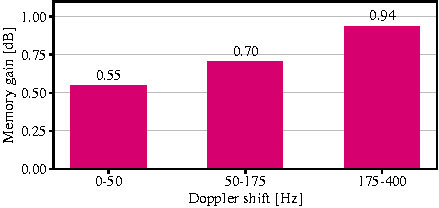
\includegraphics[width=\columnwidth]{figures/memory_gain_vs_doppler.pdf}
\caption{Memory gain in effective SNR at a TBLER of 10\% vs.\ Doppler shift for UMi.}
\label{fig:doppler}
\end{figure}

These gains, however, depend strongly on the channel speed. Fig.~\ref{fig:doppler} shows the memory gain for UMi, grouped by Doppler shift. To remove the effect of low channel power, we evaluate TBLER against the effective SNR, i.e., the SNR plus the effective channel power of the UE in dB. The gain at a TBLER of 10\% is 0.06\,dB for 0--50\,Hz, 0.20\,dB for 50--175\,Hz, and 1.25\,dB for 175--400\,Hz. On slow channels, the proposed NRX with no memory already matches Perf.-CSI + K-Best, leaving little room for improvement by the memory. Each group contains about 10 sequences, so these values are indicative.

We confirm the memory gain on two further independent evaluation datasets at a fixed SNR per condition, chosen for a TBLER near 10\% for the Large NRX on separate data. They also include closely spaced line-of-sight (LOS) UEs, at most $5^\circ$ apart in azimuth, near-far UEs with a received power difference of 6 or 12\,dB, and, on one dataset, channels ray-traced with Sionna RT~\cite{hoydis2023} in the Munich scene of \citet{wiesmayr2024}. The memory lowers TBLER in all of these cases except for closely spaced LOS UEs on one dataset, where it is unchanged, while the Large NRX remains ahead of the proposed NRX in some cases.

\subsection{Latency}
Fig.~\ref{fig:tradeoff} shows the required SNR and median latency for UMi. We time 128 TBs at an SNR of 3\,dB, one TB at a time, in TensorFlow on an NVIDIA A40 GPU. The measurement covers everything after the initial LS estimation and interpolation, including LDPC decoding, CRC, and memory transfers between host and device. These values are not comparable with the real-time budget of 1\,ms in \citet{wiesmayr2024}, which covers neural network inference with TensorRT on an NVIDIA A100 GPU, and our implementation is not real-time capable.

\begin{figure}[!ht]
\centering
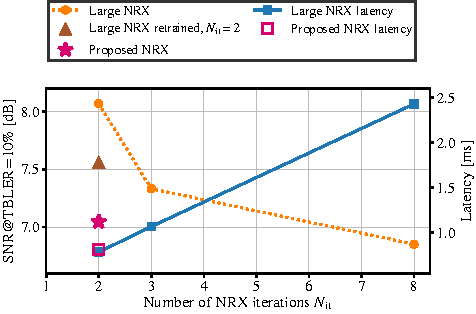
\includegraphics[width=\columnwidth]{figures/snr_latency_tradeoff.pdf}
\caption{SNR performance and median latency vs.\ number of NRX iterations for UMi.}
\label{fig:tradeoff}
\end{figure}

The proposed NRX has a median latency of 41.27\,ms (41.16\,ms with no memory), compared with 40.59\,ms, 43.09\,ms, and 53.05\,ms for the Large NRX with $N_{\mathrm{it}}=2$, 3, and 8, respectively. This is 0.68\,ms more than the Large NRX with $N_{\mathrm{it}}=2$ and 22\% less than with $N_{\mathrm{it}}=8$, at a comparable required SNR.

All results are obtained from simulations with a single training seed.

% The workshop connection and the Discussion are intentionally not started yet.

\bibliography{references}

% Optional appendix: follows the references and is outside the workshop page limit.
% \appendix
% \section{Receiver Architecture Details}

% Reproducibility checklist from the AAAI-27 kit. Not printed: the workshop page does not
% say it is required. To include it, change \iffalse to \iftrue.
\iffalse
\setlength{\leftmargini}{20pt}
\makeatletter\def\@listi{\leftmargin\leftmargini \topsep .5em \parsep .5em \itemsep .5em}
\def\@listii{\leftmargin\leftmarginii \labelwidth\leftmarginii \advance\labelwidth-\labelsep \topsep .4em \parsep .4em \itemsep .4em}
\def\@listiii{\leftmargin\leftmarginiii \labelwidth\leftmarginiii \advance\labelwidth-\labelsep \topsep .4em \parsep .4em \itemsep .4em}\makeatother

\setcounter{secnumdepth}{0}
\renewcommand\thesubsection{\arabic{subsection}}
\renewcommand\labelenumi{\thesubsection.\arabic{enumi}}

\newcounter{checksubsection}
\newcounter{checkitem}[checksubsection]

\newcommand{\checksubsection}[1]{%
  \refstepcounter{checksubsection}%
  \paragraph{\arabic{checksubsection}. #1}%
  \setcounter{checkitem}{0}%
}

\newcommand{\checkitem}{%
  \refstepcounter{checkitem}%
  \item[\arabic{checksubsection}.\arabic{checkitem}.]%
}
\newcommand{\question}[2]{\normalcolor\checkitem #1 #2 \color{blue}}
\newcommand{\ifyespoints}[1]{\makebox[0pt][l]{\hspace{-15pt}\normalcolor #1}}

\section*{Reproducibility Checklist}

\vspace{1em}
\hrule
\vspace{1em}

\textbf{Instructions for Authors:}

This document outlines key aspects for assessing reproducibility. Please provide your input by editing this \texttt{.tex} file directly.

For each question (that applies), replace the ``Type your response here'' text with your answer.

\vspace{1em}
\noindent
\textbf{Example:} If a question appears as
%
\begin{center}
\noindent
\begin{minipage}{.9\linewidth}
\ttfamily\raggedright
\string\question \{Proofs of all novel claims are included\} \{(yes/partial/no)\} \\
Type your response here
\end{minipage}
\end{center}
you would change it to:
\begin{center}
\noindent
\begin{minipage}{.9\linewidth}
\ttfamily\raggedright
\string\question \{Proofs of all novel claims are included\} \{(yes/partial/no)\} \\
yes
\end{minipage}
\end{center}
%
Please make sure to:
\begin{itemize}\setlength{\itemsep}{.1em}
\item Replace ONLY the ``Type your response here'' text and nothing else.
\item Use one of the options listed for that question (e.g., \textbf{yes}, \textbf{no}, \textbf{partial}, or \textbf{NA}).
\item \textbf{Not} modify any other part of the \texttt{\string\question} command or any other lines in this document.\\
\end{itemize}

You can \texttt{\string\input} this .tex file right before \texttt{\string\end\{document\}} of your main file or compile it as a stand-alone document. Check the instructions on your conference's website to see if you will be asked to provide this checklist with your paper or separately.

\vspace{1em}
\hrule
\vspace{1em}

% The questions start here

\checksubsection{General Paper Structure}
\begin{itemize}

\question{Includes a conceptual outline and/or pseudocode description of AI methods introduced}{(yes/partial/no/NA)}
Type your response here

\question{Clearly delineates statements that are opinions, hypothesis, and speculation from objective facts and results}{(yes/no)}
Type your response here

\question{Provides well-marked pedagogical references for less-familiar readers to gain background necessary to replicate the paper}{(yes/no)}
Type your response here

\end{itemize}
\checksubsection{Theoretical Contributions}
\begin{itemize}

\question{Does this paper make theoretical contributions?}{(yes/no)}
Type your response here

	\ifyespoints{\vspace{1.2em}If yes, please address the following points:}
        \begin{itemize}
	
	\question{All assumptions and restrictions are stated clearly and formally}{(yes/partial/no)}
	Type your response here

	\question{All novel claims are stated formally (e.g., in theorem statements)}{(yes/partial/no)}
	Type your response here

	\question{Proofs of all novel claims are included}{(yes/partial/no)}
	Type your response here

	\question{Proof sketches or intuitions are given for complex and/or novel results}{(yes/partial/no)}
	Type your response here

	\question{Appropriate citations to theoretical tools used are given}{(yes/partial/no)}
	Type your response here

	\question{All theoretical claims are demonstrated empirically to hold}{(yes/partial/no/NA)}
	Type your response here

	\question{All experimental code used to eliminate or disprove claims is included}{(yes/no/NA)}
	Type your response here
	
	\end{itemize}
\end{itemize}

\checksubsection{Dataset Usage}
\begin{itemize}

\question{Does this paper rely on one or more datasets?}{(yes/no)}
Type your response here

\ifyespoints{If yes, please address the following points:}
\begin{itemize}

	\question{A motivation is given for why the experiments are conducted on the selected datasets}{(yes/partial/no/NA)}
	Type your response here

	\question{All novel datasets introduced in this paper are included in a data appendix}{(yes/partial/no/NA)}
	Type your response here

	\question{All novel datasets introduced in this paper will be made publicly available upon publication of the paper with a license that allows free usage for research purposes}{(yes/partial/no/NA)}
	Type your response here

	\question{All datasets drawn from the existing literature (potentially including authors' own previously published work) are accompanied by appropriate citations}{(yes/no/NA)}
	Type your response here

	\question{All datasets drawn from the existing literature (potentially including authors' own previously published work) are publicly available}{(yes/partial/no/NA)}
	Type your response here

	\question{All datasets that are not publicly available are described in detail, with explanation why publicly available alternatives are not scientifically satisficing}{(yes/partial/no/NA)}
	Type your response here

\end{itemize}
\end{itemize}

\checksubsection{Computational Experiments}
\begin{itemize}

\question{Does this paper include computational experiments?}{(yes/no)}
Type your response here

\ifyespoints{If yes, please address the following points:}
\begin{itemize}

	\question{This paper states the number and range of values tried per (hyper-) parameter during development of the paper, along with the criterion used for selecting the final parameter setting}{(yes/partial/no/NA)}
	Type your response here

	\question{Any code required for pre-processing data is included in the appendix}{(yes/partial/no)}
	Type your response here

	\question{All source code required for conducting and analyzing the experiments is included in a code appendix}{(yes/partial/no)}
	Type your response here

	\question{All source code required for conducting and analyzing the experiments will be made publicly available upon publication of the paper with a license that allows free usage for research purposes}{(yes/partial/no)}
	Type your response here
        
	\question{All source code implementing new methods have comments detailing the implementation, with references to the paper where each step comes from}{(yes/partial/no)}
	Type your response here

	\question{If an algorithm depends on randomness, then the method used for setting seeds is described in a way sufficient to allow replication of results}{(yes/partial/no/NA)}
	Type your response here

	\question{This paper specifies the computing infrastructure used for running experiments (hardware and software), including GPU/CPU models; amount of memory; operating system; names and versions of relevant software libraries and frameworks}{(yes/partial/no)}
	Type your response here

	\question{This paper formally describes evaluation metrics used and explains the motivation for choosing these metrics}{(yes/partial/no)}
	Type your response here

	\question{This paper states the number of algorithm runs used to compute each reported result}{(yes/no)}
	Type your response here

	\question{Analysis of experiments goes beyond single-dimensional summaries of performance (e.g., average; median) to include measures of variation, confidence, or other distributional information}{(yes/no)}
	Type your response here

	\question{The significance of any improvement or decrease in performance is judged using appropriate statistical tests (e.g., Wilcoxon signed-rank)}{(yes/partial/no)}
	Type your response here

	\question{This paper lists all final (hyper-)parameters used for each model/algorithm in the paper’s experiments}{(yes/partial/no/NA)}
	Type your response here


\end{itemize}
\end{itemize}
\fi

\end{document}
